\section{Profiling performance and power consumption}

For the perception algorithm, the first stage of our method is profiling the performance (timing and, if available, quality) and power consumption of the computation. 
To do this profiling, we first navigate the robot manually in corridors and log video from the on-board camera at a high frame-rate. 
We run Vanishing point on this video offline and profile it with different scheduling of the three components (Blur, Canny and Hough) on the CPU and GPU, and at different frequencies of both processors (Fig. \ref{fig:vanishing}).

We wrote a custom C-code library to log power measurements from a Tektronix PWS4205 Programmable DC power supply at 100Hz. 
For this we communicate with the power supply over USB using the USB Test and Measurement Class (USB-TMC) communication protocol. 

%In order to profile the timing performance of the Vanishing point algorithm with different schedules for the three tasks we allocate on either the CPU or the GPU, and the different clock frequencies for the CPU and the GPU, we have a script that runs the vanishing point algorithm for all settings offline and logs the update rate in Hz as well as individual execution times of the components and the power consumption. 
Since for an algorithm like Vanishing point there is no well-defined notion of ground truth, we do not have a measure of accuracy of the algorithm. 
Instead, the vanishing point algorithm's update rate is used as a performance measure, since with faster updates the controller can apply input signals to the car faster, resulting in better control performance. 

Figures \ref{fig:diff freq same assignment}, \ref{fig:same freq diff assignment} show the profiling results.
\begin{figure}[t]
\centering
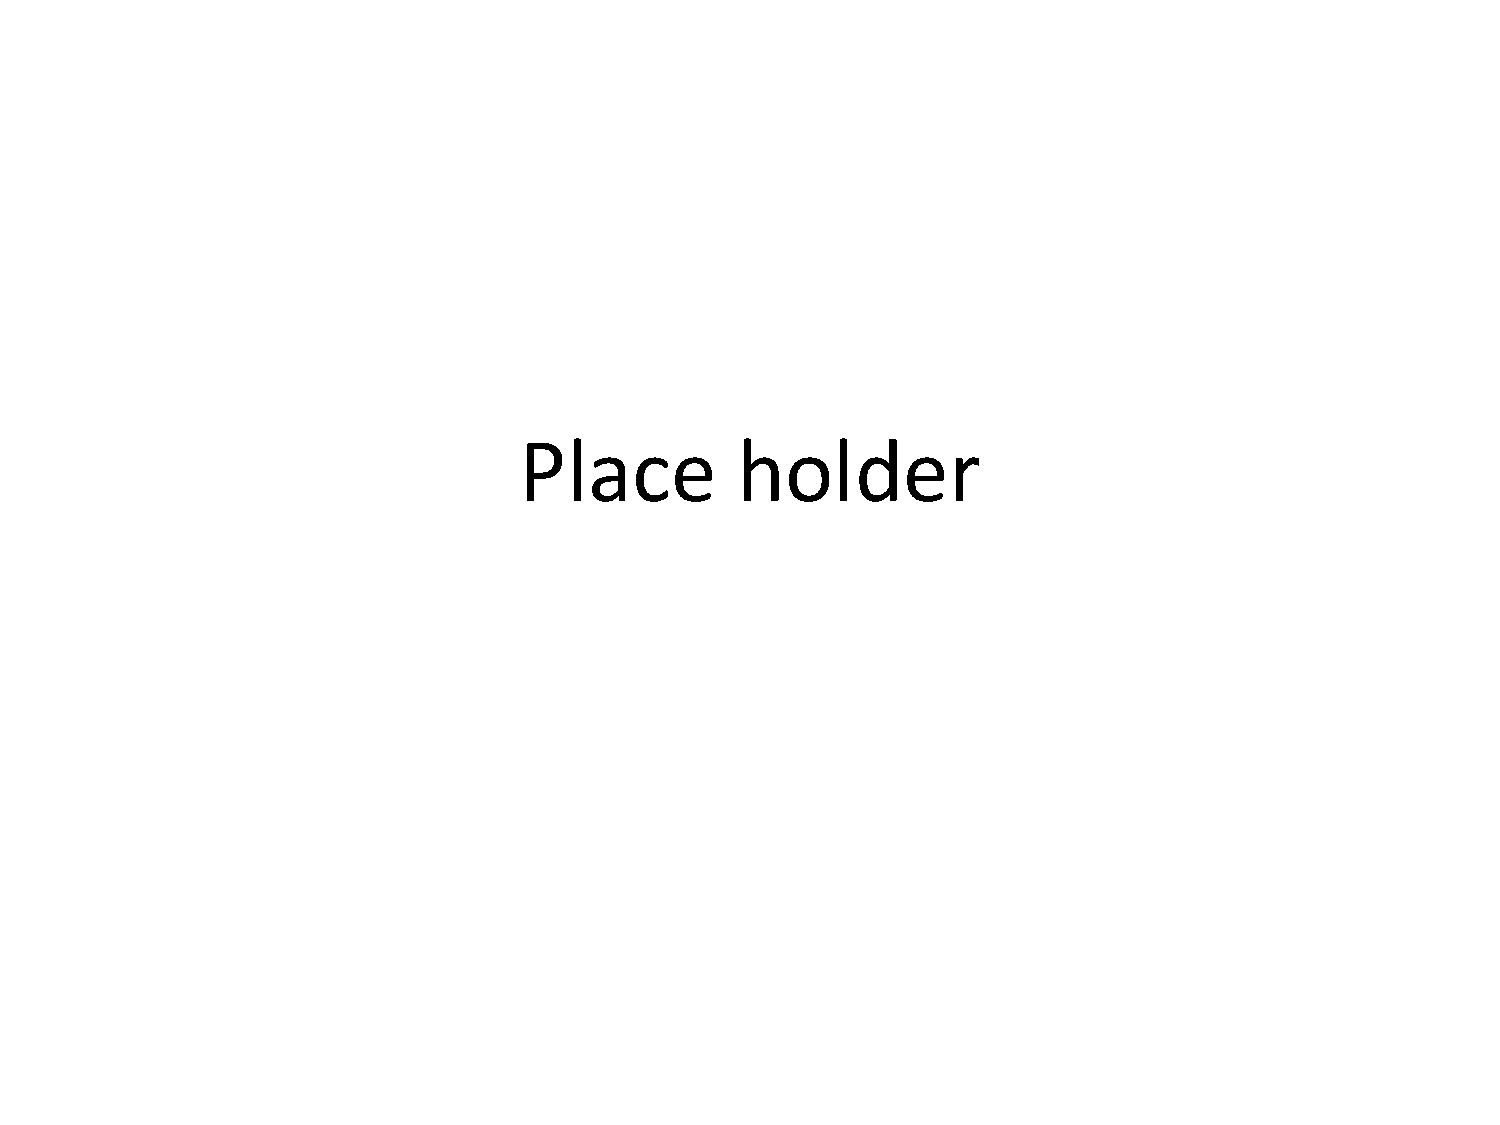
\includegraphics[scale=0.2]{Figs/placeHolder}
\caption{Update rate for different frequencies and a given CPU-GPU assignment.}
\label{fig:diff freq same assignment}
\end{figure}

\begin{figure}[t]
	\centering
	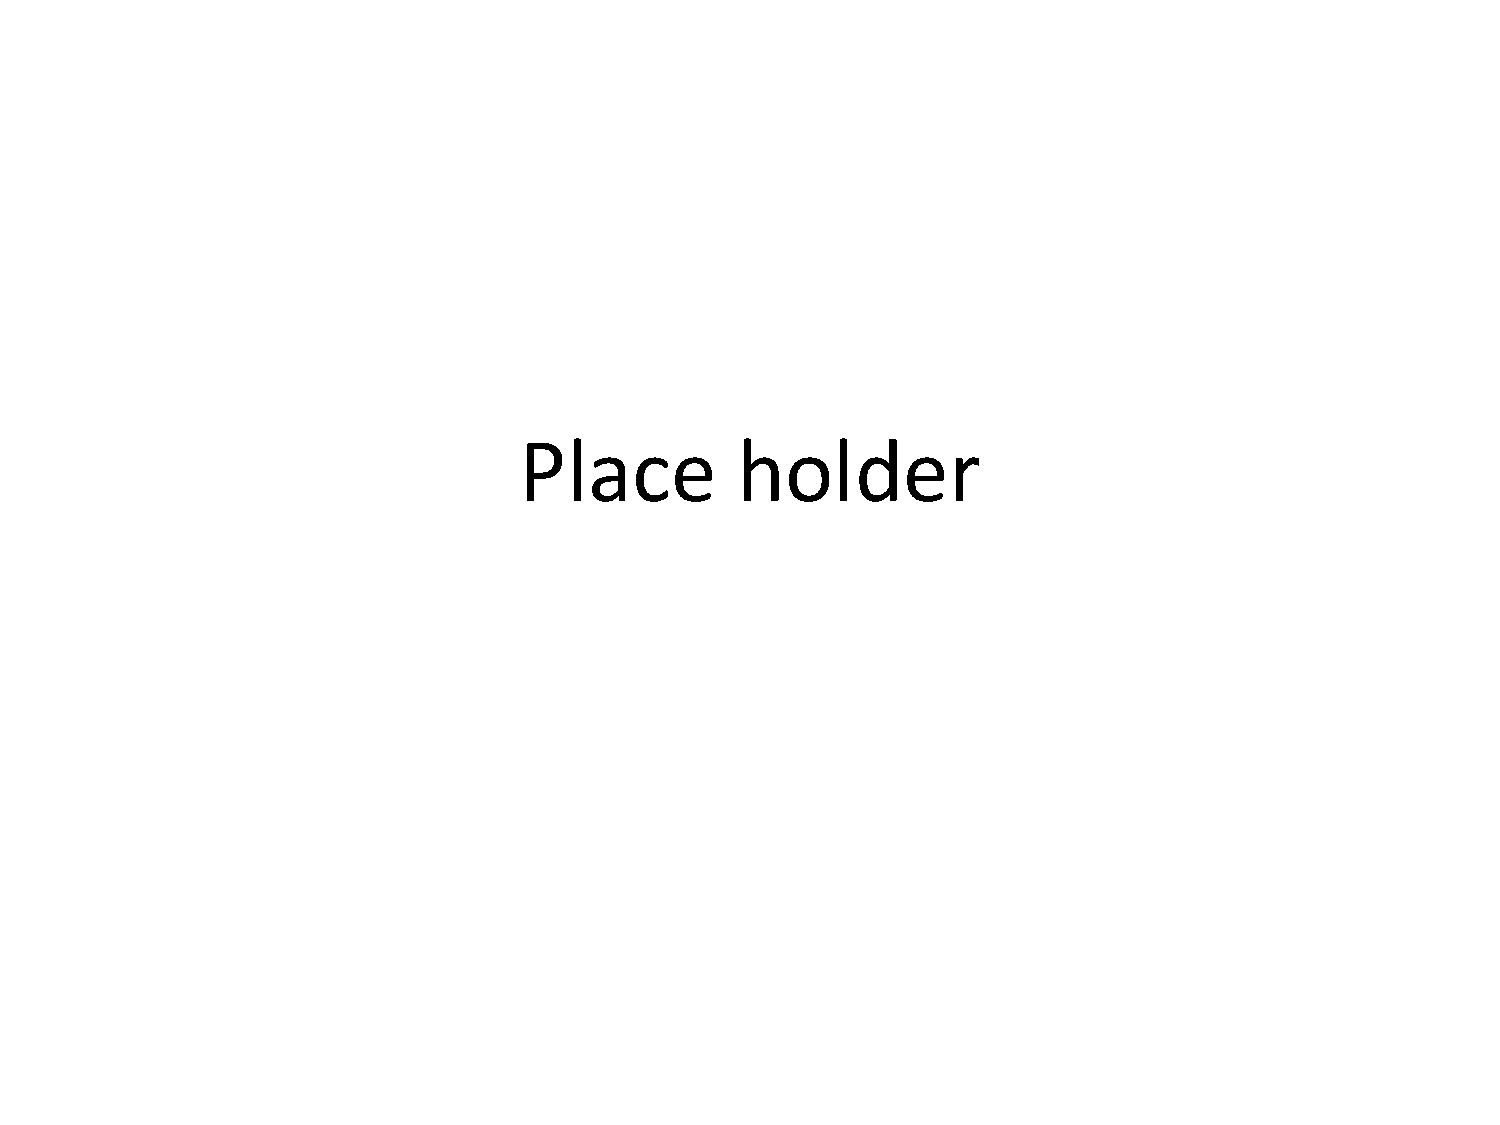
\includegraphics[scale=0.2]{Figs/placeHolder}
	\caption{Update rate for different CPU-GPU assignments at fixed frequencies.}
	\label{fig:same freq diff assignment}
\end{figure}